\subsection{\Glsfmtlong{gpt}}

\Gls{gpt} est un \gls{llm} de OpenAI~\cite{Radford_Narasimhan_Salimans_Sutskever}.
Un modèle de langage est une loi de probabilité \(\prob\) sur les phrases d'une langue~\cite{routledge}.
Dans le cas de \gls{gpt}, cette loi est calculée par un réseau de neurones.
Plus précisément, il s'agit d'une \emph{pile de décodeurs de transformeur}%
\footnote{%
    Une composition de \(N\) modules de décodeur. 
    Dans~\cite{Radford_Narasimhan_Salimans_Sutskever}, \(N=12\)
    (117M paramètres).
} (voir Figure~\ref{fig.gpt}).

\begin{figure}[hbt]
    \centering
    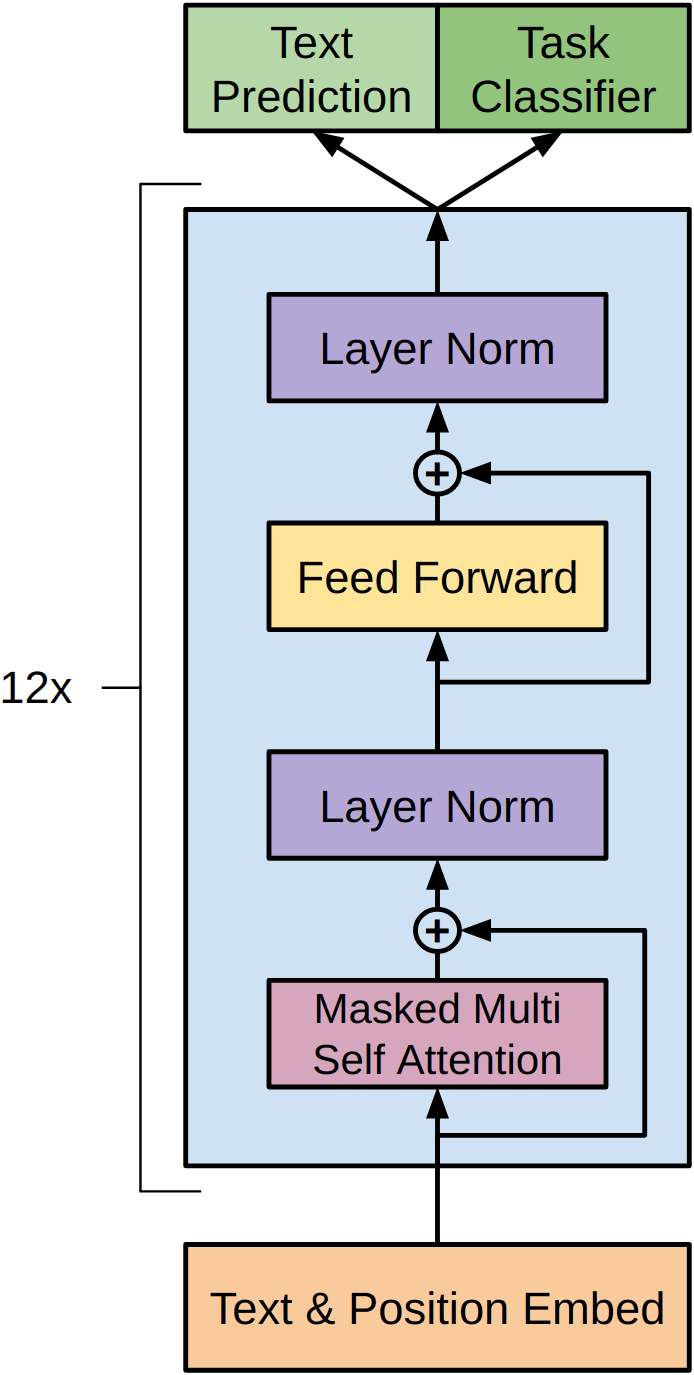
\includegraphics[height=.5\linewidth]{assets/images/gpt.png}
    \caption[Architecture de \glsfmtshort{gpt}.]%
    {Architecture de \glsfmtshort{gpt}~\cite{Radford_Narasimhan_Salimans_Sutskever}.}
    \label{fig.gpt}
\end{figure}

L'entraînement de \gls{gpt} passe par deux étapes.
Dans un premier temps, il est pré-entraîné d'une façon autosupervisée sur un corpus de texte brut.
Puis, il est affiné sur un corpus de texte annoté.
Cette deuxième étape est un exemple d'apprentissage supervisé classique.
La première est beaucoup plus intéressante.
Pendant cette étape, le modèle est entraîné sur la tâche de \gls{clm}
i.e, la tâche de prédire, à partir d'une suite de tokens, le token suivant%
~\cite{Radford_Narasimhan_Salimans_Sutskever}.
Plus exactement, le modèle est entraîné pour maximiser la fonction :
\begin{equation}
    \label{eq.gpt-pretrain-loss}
    L_1=\sum_{i=k+1}^{n-k} \log\prob{\left(t_i \mid t_{i-k}, \ldots, t_{i-1} ; \theta\right)}
\end{equation}
où \(\left(t_1, t_2, \ldots, t_n\right)\) est un corpus de taille \(n\), 
\(k\) est un hyperparamètre qui détermine la taille de la fenêtre de contexte
et \(\theta\) représente les paramètres entraînables du modèle.

Le succès de \gls{gpt} a motivé la création de plusieurs variantes.
Notamment, \gls{gpt}--2~\cite{Radford_Wu_Child_Luan_Amodei_Sutskever_2019} 
et \gls{gpt}--3~\cite{Brown_Mann_Ryder_Subbiah_Kaplan_Dhariwal_Neelakantan_Shyam_Sastry_Askell_etal._2020}.
La principale différence entre ces variantes est la taille du modèle (1.5 B et 175B paramètres respectivement).
Un autre modèle basé sur \gls{gpt} (plus précisément sur \gls{gpt}--2) 
qui est très pertinent pour notre travail est \gls{gpt}--D.
Il s'agit d'une copie de \gls{gpt}--2 dont les paramètres ont été délibérément dégradés
à fin de modéliser les erreurs linguistiques associées à la démence~\cite{Li_Knopman_Xu_Cohen_Pakhomov_2022}.